% Provenance (never printed): old premiere S material on magmatic rocks (volcanic
% and plutonic textures and cooling rate; basalt/gabbro, andesite/diorite,
% rhyolite/granite; order of crystallisation, told). Cooling of sheets from
% figdata/grade-11/dyke_cooling.py (Delaney 1986 parameters; kappa from England
% et al. 2007). Fractional crystallisation is Year 2's; metamorphism (contact
% aureoles) is g12.03's: not developed here.
\chapter{الصخور النارية}\label{ch:g11:igneous-rocks}

على الساحل الشمالي لأيرلندا، تنحدر أعمدة حجرية متراصة جنبًا إلى جنب
نحو البحر: إنها جسر العملاق، من بازلت
برد من لابة. وفي يوسميتي، في كاليفورنيا، يرتفع جدار إل كابيتان
الغرانيتي نحو \qty{900}{m} فوق قاع الوادي، وهو جسم واحد من
صخر خشن الحبيبات. وكلاهما تبلور من صهارة. فالبازلت برد على
السطح، وبلوراته أصغر من أن تُرى؛ والغرانيت برد عميقًا تحت الأرض،
وبلوراته كبيرة بما يكفي لتُرى، ولا يظهر اليوم إلا لأن
الصخور التي كانت فوقه قد تآكلت. يقرأ هذا الفصل في حبيبات الصخر
مدى سرعة تبرده، وعلى أي عمق برد.
% ledger: photo:g11-giants-causeway, photo:g11-el-capitan, tulane:intrusions

\begin{omfigure}
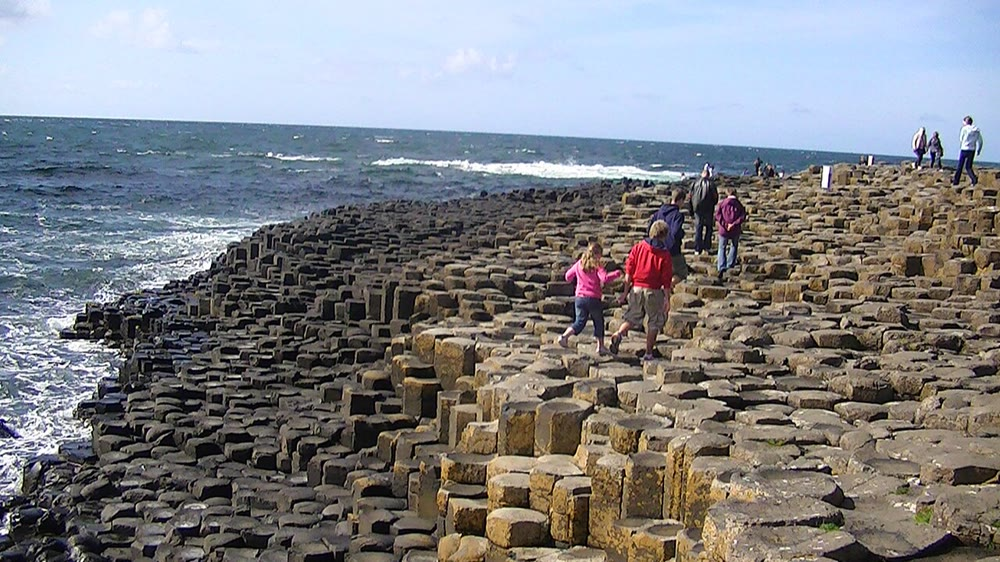
\includegraphics[height=4.3cm]{images/book2/g11-bishop-giants-causeway.jpg}\hspace{0.04\linewidth}%
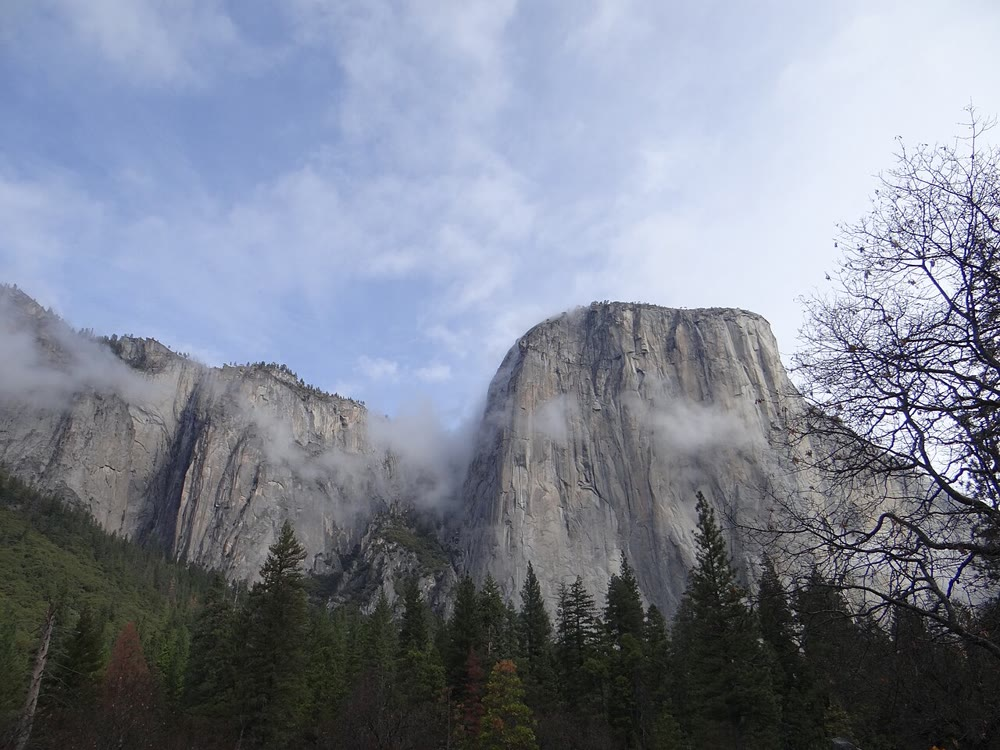
\includegraphics[height=4.3cm]{images/book2/g11-usgs-el-capitan.jpg}

{\small في اليمين: أعمدة البازلت في جسر العملاق، في أيرلندا الشمالية.
الصورة: آدم بيشوب (\babelsublr{CC~BY-SA~3.0}). في اليسار: إل كابيتان، يوسميتي،
كاليفورنيا، جدار من الغرانيت ارتفاعه نحو \qty{900}{m}. الصورة: هيئة المسح
الجيولوجي الأمريكية (\babelsublr{CC0}).}
\end{omfigure}
% ledger: photo:g11-giants-causeway, photo:g11-el-capitan

\begin{recall}
الصهارة صخر منصهر تحت السطح؛ وتنبثق لابةً، بهدوء أو
بانفجار (الكتاب 1، الصف 7). والصخر الناري صخر تكوّن حين برد صخر
منصهر وتصلب (الكتاب 1، الصف 6). والبازلت \omterm{def:g11:igneous-rocks:volcanic-plutonic}{صخر بركاني} داكن، والغرانيت
صخر فاتح يتكون من الفلسبار والكوارتز والميكا (الكتاب 1، الصف 6). \omterm{def:g11:ocean-ridges:peridotite}{وبيريدوتيت}
الوشاح ينصهر جزئيًا وهو يصعد تحت الظهرة، فيعطي بازلت \omterm{def:g11:ocean-ridges:oceanic-lithosphere}{القشرة المحيطية}
وغابروها (\cref{ch:g11:ocean-ridges}). \omterm{def:g11:minerals:rock-forming}{والسيليكات المكوّنة
للصخور} هي الأوليفين والبيروكسينات والأمفيبولات والميكا والفلسبارات والكوارتز؛
والفلسبارات هي فلسبار البوتاسيوم والبلاجيوكليز، وهو سلسلة تمتد من
الغني بالكالسيوم إلى الغني بالصوديوم (\cref{ch:g11:minerals}). وتنتشر الحرارة
بالتوصيل على مسافة قدرها نحو $\sqrt{\kappa t}$ في زمن $t$، حيث
$\kappa$ هو الانتشارية الحرارية (\cref{ch:g11:subduction-zones}).
\end{recall}
% ledger: tulane:ridge-rocks, england:kelvin

\section{الصخور البركانية والصخور الجوفية}

\begin{definition}[الصخر البركاني؛ الصخر الجوفي]\label{def:g11:igneous-rocks:volcanic-plutonic}
الصخر الناري، المتكوّن بتبلور صهارة، يكون
\emph{بركانيًا}\index{صخر بركاني}
(أو انبثاقيًا) حين تكون الصهارة قد تصلبت على سطح الأرض، لابةً،
و\emph{جوفيًا}\index{صخر جوفي} (أو متداخلًا) حين تكون قد تبلورت
في العمق، داخل صخور أخرى.
\end{definition}
% ledger: tulane:magma-types

يظهر الفرق في حجم البلورات. فالبلورة تنمو بإضافة
ذرات تأخذها من السائل المحيط بها، وهذا يستغرق وقتًا. وعلى السطح
تفقد اللابة حرارتها في الهواء أو الماء بسرعة: فالمواد المقذوفة في الهواء أو
الماء تبرد في ثوانٍ، والمسيل اللابي في أيام إلى أسابيع. أما في العمق فتكون
الصخور المحيطة ساخنة وتفقد الصهارة حرارتها ببطء: \omterm{def:g11:igneous-rocks:intrusion}{فالجسم المتداخل}
الضحل يبرد في أشهر إلى سنوات، وقد يستغرق الجسم الكبير العميق ملايين
السنين. والتبرد السريع يعطي بلورات صغيرة كثيرة، أو لا يعطي بلورات أصلًا؛ والتبرد البطيء
يعطي بلورات أقل عددًا وأكبر بكثير.
% ledger: tulane:cooling-times, tulane:textures

\begin{definition}[النسيج]\label{def:g11:igneous-rocks:texture}
\emph{نسيج}\index{نسيج (الصخر)} الصخر هو حجم حبيباته وشكلها
وترتيبها. ويكون الصخر الناري \emph{زجاجيًا} حين
لا تكون فيه بلورات، و\emph{دقيق الحبيبات} حين تكون بلوراته أصغر من أن
تُميَّز بالعين المجردة، و\emph{خشن الحبيبات} حين تُرى
كلها.
\end{definition}
% ledger: tulane:textures

اللابة التي تُخمد فجأة قبل أن تنمو أي بلورة تصير زجاجًا: فالأوبسيديان، الأسود
الزجاجي، ينكسر \omterm{def:g11:minerals:cleavage}{بالمكسر} المحاري للقارورة. والبازلت
دقيق الحبيبات: لا يمكن تعرّف معادنه باليد، وحتى في
\omterm{def:g11:minerals:thin-section}{الشريحة الرقيقة} تكون البلورات صغيرة (بازلت \cref{ch:g11:minerals}).
أما الغرانيت \omterm{def:g11:ocean-ridges:gabbro}{والغابرو} \omterm{def:g11:igneous-rocks:rock-names}{والديوريت} فخشنة الحبيبات: كل حبيبة فيها تُرى.
% ledger: photo:g11-obsidian, photo:g11-basalt, tulane:textures

\begin{definition}[البلورة الظاهرة؛ البورفيري]\label{def:g11:igneous-rocks:porphyritic}
\emph{البلورة الظاهرة}\index{بلورة ظاهرة} بلورة كبيرة مغروسة في كتلة من
بلورات أصغر بكثير أو من الزجاج، تسمى \emph{الأرضية}. والصخر الذي فيه
بلورات ظاهرة صخر \emph{بورفيري}\index{بورفيري}.
\end{definition}
% ledger: tulane:textures

يسجّل \omterm{def:g11:igneous-rocks:texture}{النسيج} \omterm{def:g11:igneous-rocks:porphyritic}{البورفيري} مرحلتين من التبرد: الأولى بطيئة، في العمق،
نمت خلالها \omterm{def:g11:igneous-rocks:porphyritic}{البلورات الظاهرة} في صهارة كانت لا تزال سائلة في معظمها؛ ثم
سريعة، حين صعدت الصهارة وانبثقت، أو حُقنت في صخر بارد،
وتجمّد ما بقي من السائل فصار الأرضية.
% ledger: tulane:textures

\begin{omfigure}
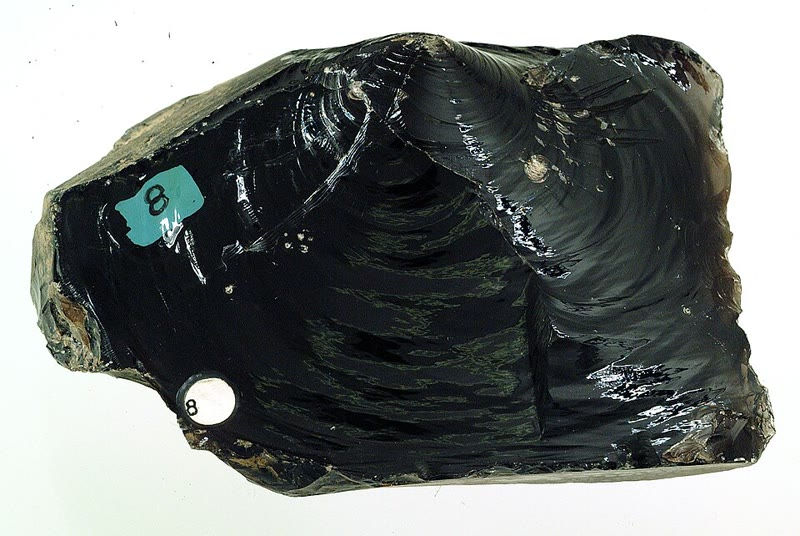
\includegraphics[height=2.75cm]{images/book2/g11-geodil-obsidian.jpg}\hfill
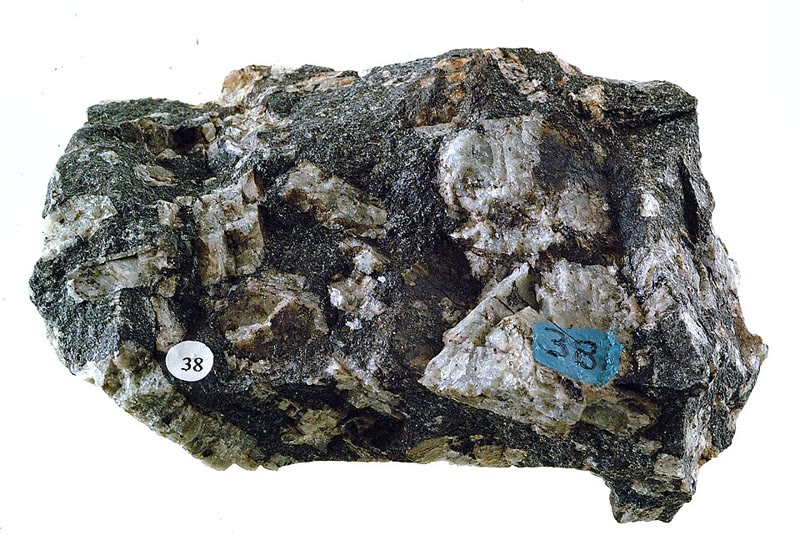
\includegraphics[height=2.75cm]{images/book2/g11-geodil-diabase-porphyry.jpg}\hfill
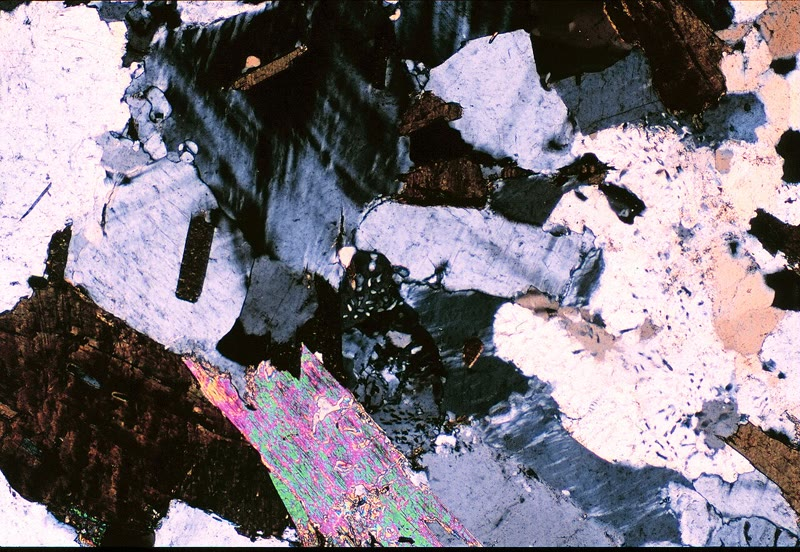
\includegraphics[height=2.75cm]{images/book2/g11-geodil-granite-xpl.jpg}\hfill
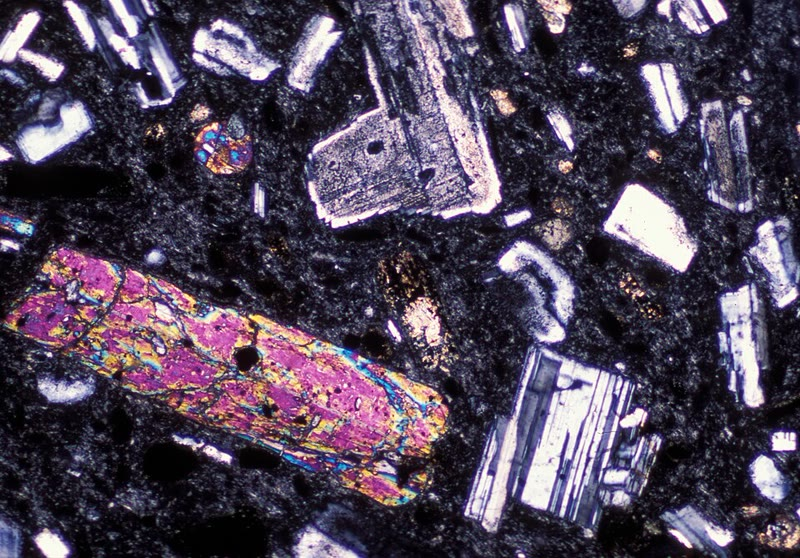
\includegraphics[height=2.75cm]{images/book2/g11-geodil-andesite-xpl.jpg}

{\small من اليمين إلى اليسار: الأوبسيديان، وهو \omterm{def:g11:igneous-rocks:volcanic-plutonic}{زجاج بركاني}، بمكسره المحاري
المنحني (عرضه \qty{9.5}{cm})؛ وصخر \omterm{def:g11:igneous-rocks:porphyritic}{بورفيري}، فيه \omterm{def:g11:igneous-rocks:porphyritic}{بلورات ظاهرة} كتلية من
البلاجيوكليز في أرضية أدق (\qty{9}{cm})؛ ثم شريحتان
رقيقتان بين المستقطبين المتعامدين: غرانيت، حبيباته كلها كبيرة
ومتشابكة --- بيوتيت بني، ومسكوفيت زاهي الألوان، وبلاجيوكليز
مخطط، وكوارتز رمادي وأبيض؛ \omterm{def:g11:igneous-rocks:rock-names}{وأنديزيت}، فيه \omterm{def:g11:igneous-rocks:porphyritic}{بلورات ظاهرة} من
البلاجيوكليز والأمفيبول في أرضية دقيقة الحبيبات. الصور: تويلا
بيكر ومايك ديفيس ودارلا سوندرول، المكتبة الرقمية لصور الجيولوجيا (\babelsublr{CC0}).}
\end{omfigure}
% ledger: photo:g11-obsidian, photo:g11-diabase-porphyry, photo:g11-granite-xpl, photo:g11-andesite-xpl

\section{تسمية الصخور النارية}

المفتاح الثاني للصخر الناري هو كيمياؤه، وقبل كل شيء
محتواه من السيليكا، \ce{SiO2}، الذي يتراوح في الصهارات الشائعة من نحو
\qty{45}{\percent} إلى نحو \qty{75}{\percent} من الكتلة.

\begin{definition}[المافي؛ المتوسط؛ الفلسي]\label{def:g11:igneous-rocks:felsic-mafic}
تكون الصهارة، أو الصخر الذي تكوّنه، \emph{مافية}\index{مافي} حين تحتوي على
نحو \qty{45}{\percent} إلى \qty{55}{\percent} من \ce{SiO2} وتكون غنية
بالحديد والمغنيسيوم والكالسيوم؛ و\emph{متوسطة}\index{متوسط (صخر)}
بين \qty{55}{\percent} و\qty{65}{\percent}؛ و\emph{فلسية}\index{فلسي}
حين تحتوي على نحو \qty{65}{\percent} إلى \qty{75}{\percent} من \ce{SiO2} وتكون
فقيرة بالحديد والمغنيسيوم والكالسيوم لكنها غنية بالصوديوم والبوتاسيوم.
\end{definition}
% ledger: tulane:magma-types, earle:magma-oxides

كل نوع من الصهارة يعطي صخرين، أحدهما بركاني دقيق الحبيبات، والآخر
جوفي خشن الحبيبات، لهما الكيمياء نفسها. فالبازلت \omterm{def:g11:ocean-ridges:gabbro}{والغابرو} هما
الزوج \omterm{def:g11:igneous-rocks:felsic-mafic}{المافي}، وقد عرفناهما مع \omterm{def:g11:ocean-ridges:oceanic-lithosphere}{القشرة المحيطية}؛ والغرانيت هو \omterm{def:g11:igneous-rocks:volcanic-plutonic}{الصخر الجوفي}
\omterm{def:g11:igneous-rocks:felsic-mafic}{الفلسي}. وثلاثة أسماء تكمل المجموعة.

\begin{definition}[الأنديزيت؛ الديوريت؛ الريوليت]\label{def:g11:igneous-rocks:rock-names}
\emph{الأنديزيت}\index{أنديزيت} و\emph{الديوريت}\index{ديوريت} هما
\omterm{def:g11:igneous-rocks:volcanic-plutonic}{الصخر البركاني} \omterm{def:g11:igneous-rocks:volcanic-plutonic}{والصخر الجوفي} ذوا التركيب المتوسط، ويتكونان في معظمهما من
البلاجيوكليز مع الأمفيبول أو البيروكسين. و\emph{الريوليت}\index{ريوليت} هو
\omterm{def:g11:igneous-rocks:volcanic-plutonic}{الصخر البركاني} ذو التركيب \omterm{def:g11:igneous-rocks:felsic-mafic}{الفلسي}، المكافئ الدقيق الحبيبات
للغرانيت.
\end{definition}
% ledger: tulane:magma-types, earle:bowen, photo:g11-andesite, photo:g11-diorite

\begin{omfigure}
\begin{tikzpicture}[font=\footnotesize, x=0.4cm]
  % columns: SiO2 45 to 75 % mapped to x = 45 to 75 (0.4 cm per %)
  \begin{scope}[xshift=-18cm]
  \fill[omLithBasalt!45] (45,0) rectangle (55,2.4);
  \fill[omLithBasalt!20] (55,0) rectangle (65,2.4);
  \fill[omLithGranite!45] (65,0) rectangle (75,2.4);
  \draw[black!60] (45,0) rectangle (75,2.4);
  \draw[black!60] (55,0) -- (55,2.4); \draw[black!60] (65,0) -- (65,2.4);
  \draw[black!60] (45,1.2) -- (75,1.2);
  \foreach \x/\a/\b in {50/البازلت/الغابرو, 60/الأنديزيت/الديوريت, 70/الريوليت/الغرانيت}{
    \node[font=\small\bfseries, text height=1.6ex, text depth=0.3ex] at (\x,1.8) {\a};
    \node[font=\small\bfseries, text height=1.6ex, text depth=0.3ex] at (\x,0.6) {\b};}
  \node[anchor=east, align=right] at (44.4,1.8) {دقيقة الحبيبات\\(بركانية)};
  \node[anchor=east, align=right] at (44.4,0.6) {خشنة الحبيبات\\(جوفية)};
  \node[anchor=south] at (50,2.45) {مافي};
  \node[anchor=south] at (60,2.45) {متوسط};
  \node[anchor=south] at (70,2.45) {فلسي};
  % minerals (a drawing: where each mineral is common)
  \foreach \y/\a/\b/\m/\c in {-0.55/45.2/52/الأوليفين/omLithBasalt!80!black,
      -1.15/45.2/61/البيروكسين/omLithBasalt!65!black,
      -1.75/52/69/الأمفيبول/black!60,
      -2.35/57/74.8/البيوتيت/black!75,
      -2.95/45.2/72/البلاجيوكليز/omDef!45,
      -3.55/63/74.8/فلسبار البوتاسيوم/omLithGranite!90!red,
      -4.15/64/74.8/الكوارتز/black!20,
      -4.75/68/74.8/المسكوفيت/black!35}{
    \fill[\c] (\a,\y) .. controls ({\a+1.2},{\y+0.22}) and ({\b-1.2},{\y+0.22}) .. (\b,\y)
              .. controls ({\b-1.2},{\y-0.22}) and ({\a+1.2},{\y-0.22}) .. (\a,\y) -- cycle;
    \node[anchor=east] at (44.4,\y) {\m};}
  \node[font=\scriptsize, text=black!75] at (50,-2.95) {غني بالكالسيوم};
  \node[font=\scriptsize, text=omDef!80!black, anchor=west] at (72.3,-2.95) {غني بالصوديوم};
  % SiO2 axis
  \draw[-{Stealth[length=4pt]}] (45,-5.35) -- (75.8,-5.35);
  \foreach \x in {45,50,...,75} {\draw (\x,-5.35) -- (\x,-5.45); \node[anchor=north] at (\x,-5.45) {\x};}
  \node[anchor=north] at (60,-5.85) {\foreignlanguage{arabic}{نسبة \babelsublr{\ce{SiO2}} من الكتلة \babelsublr{(\unit{\percent})}}};
  \draw[black!30, dashed] (55,0) -- (55,-5.35); \draw[black!30, dashed] (65,0) -- (65,-5.35);
  \end{scope}
\end{tikzpicture}

{\small تسمية الصخور النارية الشائعة (رسم). الأعمدة: محتوى
الصهارة من السيليكا؛ والصفوف: الصخور الدقيقة الحبيبات (البركانية) والخشنة الحبيبات
(الجوفية). وفي الأسفل، حيث يشيع كل معدن من المعادن المكوّنة للصخور: الأوليفين
والبيروكسين في الصخور \omterm{def:g11:igneous-rocks:felsic-mafic}{المافية} مع البلاجيوكليز الغني بالكالسيوم؛ والأمفيبول
والبلاجيوكليز في الصخور \omterm{def:g11:igneous-rocks:felsic-mafic}{المتوسطة}؛ وفلسبار البوتاسيوم والكوارتز
والبلاجيوكليز الغني بالصوديوم والميكا في الصخور \omterm{def:g11:igneous-rocks:felsic-mafic}{الفلسية}. والحدود
تدريجية.}
\end{omfigure}
% ledger: tulane:magma-types, earle:bowen, earle:magma-oxides, photo:g11-andesite, photo:g11-diorite, photo:g11-granite, nps:granite-minerals

\begin{method}[تسمية صخر ناري]\label{met:g11:igneous-rocks:naming}
\begin{enumerate}
  \item انظر إلى \omterm{def:g11:igneous-rocks:texture}{النسيج}: زجاجي، أو دقيق الحبيبات، أو خشن الحبيبات؛
        \omterm{def:g11:igneous-rocks:porphyritic}{بورفيري} أم لا. فدقيق الحبيبات أو الزجاجي يعني \omterm{def:g11:igneous-rocks:volcanic-plutonic}{بركانيًا} (أو
        \omterm{def:g11:igneous-rocks:intrusion}{جسمًا متداخلًا} صغيرًا برد بسرعة)؛ وخشن الحبيبات يعني \omterm{def:g11:igneous-rocks:volcanic-plutonic}{جوفيًا}.
  \item تعرّف المعادن التي يمكن رؤيتها
        (\cref{met:g11:minerals:identify}): فالكوارتز وفلسبار البوتاسيوم
        يدلان على \omterm{def:g11:igneous-rocks:felsic-mafic}{الفلسي}، والأمفيبول مع البلاجيوكليز على المتوسط، والأوليفين
        والبيروكسين على \omterm{def:g11:igneous-rocks:felsic-mafic}{المافي}. وفي الصخر الدقيق الحبيبات، استعمل \omterm{def:g11:igneous-rocks:porphyritic}{البلورات الظاهرة}،
        ولون الأرضية --- الداكن \omterm{def:g11:igneous-rocks:felsic-mafic}{للمافي}، والفاتح \omterm{def:g11:igneous-rocks:felsic-mafic}{للفلسي} ---
        بوصفه إشارة، أو تحليلًا كيميائيًا.
  \item اقرأ الاسم عند تقاطع الصف والعمود في
        المخطط.
\end{enumerate}
\end{method}

\begin{example}[بازلتان]
صخر داكن من مسيل لابي دقيق الحبيبات كله؛ وآخر، من
البركان نفسه، تظهر فيه حبيبات خضراء من الأوليفين عرضها بضعة مليمترات في
أرضية داكنة. كلاهما \omterm{def:g11:igneous-rocks:felsic-mafic}{مافي} ودقيق الحبيبات: فكلاهما بازلت.
والثاني بازلت \omterm{def:g11:igneous-rocks:porphyritic}{بورفيري}: فأوليفينه نما أولًا، ببطء، في
الصهارة تحت البركان، قبل أن تنبثق اللابة وتتجمد حوله.
\end{example}
% ledger: photo:g11-olivine, earle:bowen, tulane:textures

\begin{omfigure}
\makebox[0.32\linewidth]{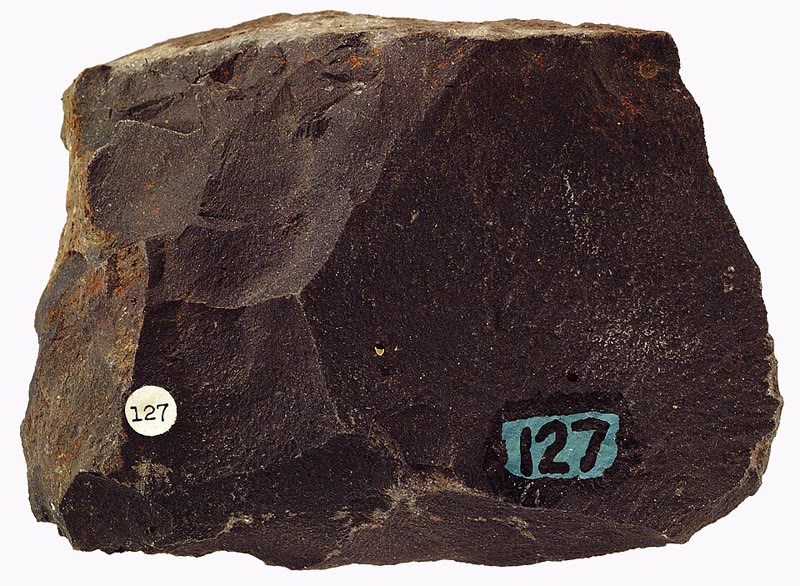
\includegraphics[height=2.9cm]{images/book2/g11-geodil-basalt.jpg}}\hfill
\makebox[0.32\linewidth]{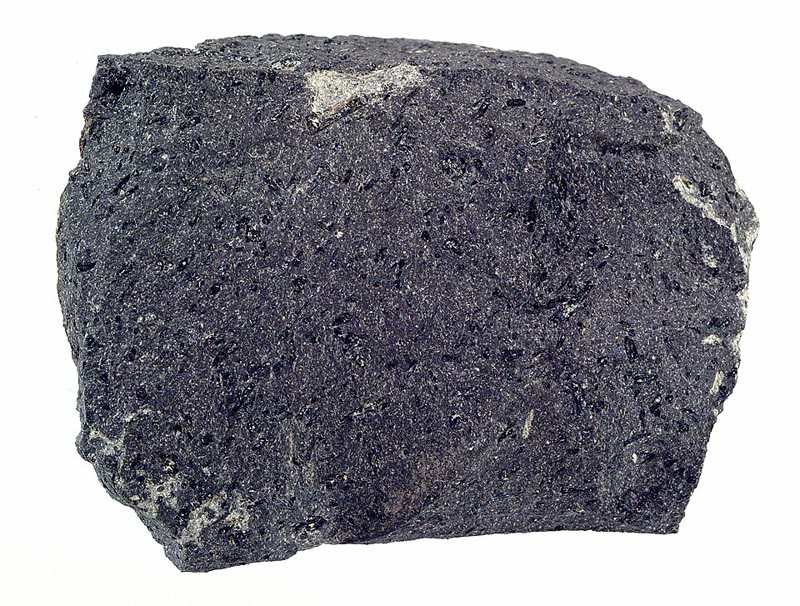
\includegraphics[height=2.9cm]{images/book2/g11-geodil-andesite.jpg}}\hfill
\makebox[0.32\linewidth]{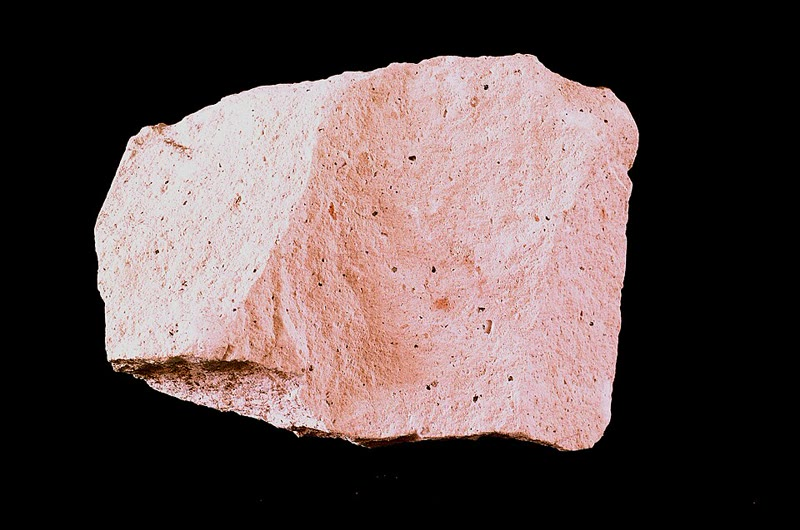
\includegraphics[height=2.9cm]{images/book2/g11-geodil-rhyolite.jpg}}

\smallskip
\makebox[0.32\linewidth]{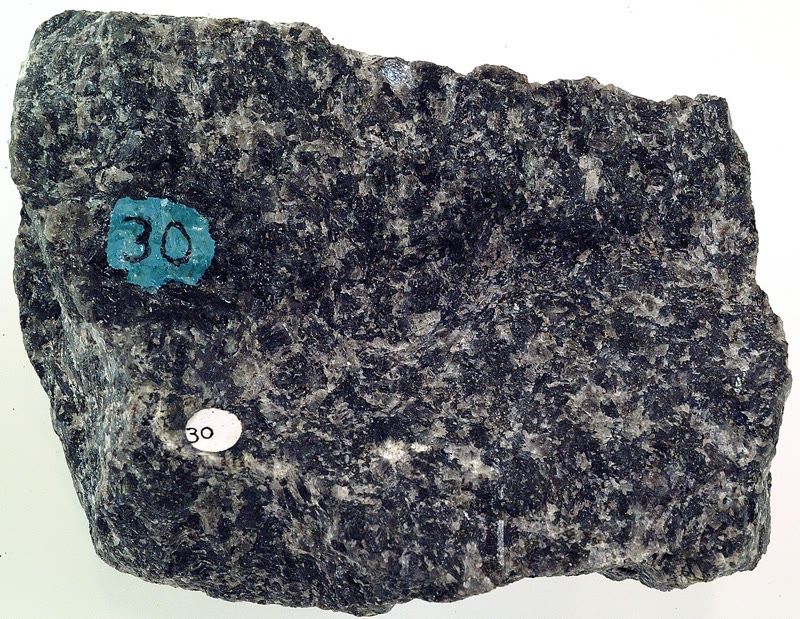
\includegraphics[height=2.9cm]{images/book2/g11-geodil-gabbro.jpg}}\hfill
\makebox[0.32\linewidth]{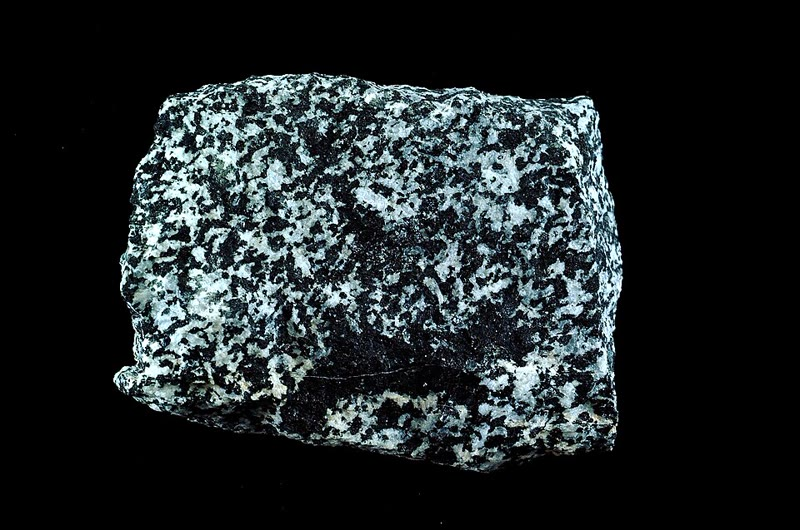
\includegraphics[height=2.9cm]{images/book2/g11-geodil-diorite.jpg}}\hfill
\makebox[0.32\linewidth]{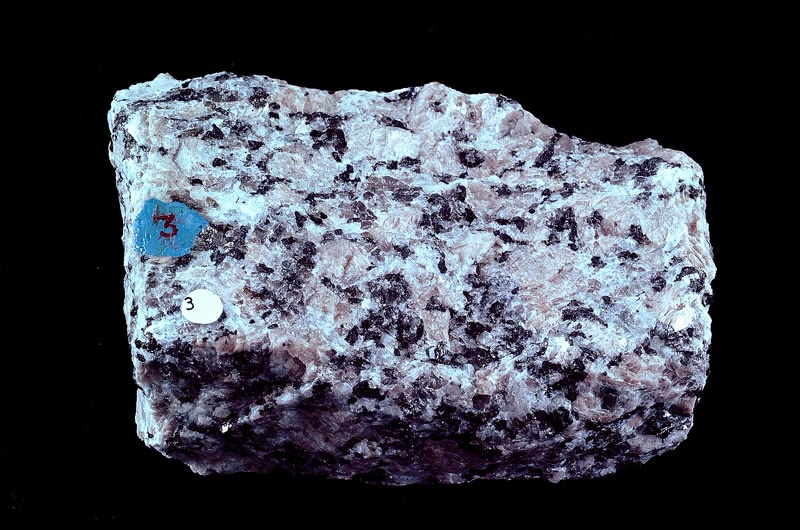
\includegraphics[height=2.9cm]{images/book2/g11-geodil-granite.jpg}}

{\small الأزواج الثلاثة من الصخور النارية، من \omterm{def:g11:igneous-rocks:felsic-mafic}{المافي} إلى \omterm{def:g11:igneous-rocks:felsic-mafic}{الفلسي} من اليمين إلى اليسار:
البركانية في الأعلى، والجوفية في الأسفل. في الأعلى: بازلت دقيق الحبيبات؛ \omterm{def:g11:igneous-rocks:rock-names}{وأنديزيت}، فيه بلورات
أمفيبول صغيرة في أرضية دقيقة الحبيبات (نحو \qty{10}{cm})؛
\omterm{def:g11:igneous-rocks:rock-names}{وريوليت} وردي. في الأسفل: \omterm{def:g11:ocean-ridges:gabbro}{غابرو} (\qty{9}{cm})؛ \omterm{def:g11:igneous-rocks:rock-names}{وديوريت}، فيه هورنبلند أسود
وبلاجيوكليز زجاجي (\qty{10}{cm})؛ وغرانيت خشن فيه بلورات كبيرة وردية فاتحة
من فلسبار البوتاسيوم، وبلاجيوكليز رمادي، وكوارتز، وبيوتيت، وهورنبلند
(\qty{10}{cm}). الصور: نيسا يول وتويلا بيكر وجوزيف إتش.~هارتمان
ودارلا سوندرول ودكستر بيركنز، المكتبة الرقمية لصور الجيولوجيا (\babelsublr{CC0}).}
\end{omfigure}
% ledger: photo:g11-basalt, photo:g11-andesite, photo:g11-rhyolite, photo:g11-gabbro, photo:g11-diorite, photo:g11-granite

\section{ترتيب التبلور}

لا تتجمد الصهارة عند درجة حرارة واحدة، كما يتجمد الماء. فمعادنها
تظهر واحدًا بعد آخر وهي تبرد، كل منها في مجاله الخاص من درجات الحرارة،
فيمكن للصهارة المتبردة أن تحوي بلورات وتبقى سائلة في معظمها.

\begin{history}[تجارب بوين]
التحق نورمان إل.~بوين (1887--1956) بالمختبر الجيوفيزيائي التابع
لمعهد كارنيغي في واشنطن عام 1912. وكان يعمل في الغالب على صهارات
بازلتية، فيصهر صخرًا في فرن، ويتركه يبرد ببطء حتى درجة حرارة
مختارة فتتكوّن بعض المعادن، ثم يُخمده فجأة، فيبرّده بسرعة
تجعل السائل المتبقي زجاجًا. وتحت المجهر كانت
البلورات تبيّن المعادن التي تكوّنت فوق تلك الدرجة. وبتكرار
التجربة عند درجات حرارة أدنى فأدنى، تبيّن الترتيب الذي تظهر به
المعادن. ونشر بوين هذا الترتيب سلسلةً تفاعلية عام 1922،
ونشر كتابه \emph{«تطور الصخور النارية»} عام 1928.
\end{history}
% ledger: carnegie:bowen, earle:bowen

\begin{omfigure}
\begin{tikzpicture}[font=\footnotesize, box/.style={draw=black!60, rounded corners=2pt, fill=#1, minimum width=3.0cm, minimum height=0.62cm, align=center}]
  \node[box=omLithBasalt!45] (ol) at (0,0) {الأوليفين};
  \node[box=omLithBasalt!35] (px) at (0,-1.1) {البيروكسين};
  \node[box=black!15] (am) at (0,-2.2) {الأمفيبول};
  \node[box=black!25] (bi) at (0,-3.3) {البيوتيت};
  \draw[-{Stealth[length=4pt]}, line width=0.8pt] (ol) -- (px);
  \draw[-{Stealth[length=4pt]}, line width=0.8pt] (px) -- (am);
  \draw[-{Stealth[length=4pt]}, line width=0.8pt] (am) -- (bi);
  \node[align=center, anchor=south] at (0,0.45) {\textbf{الفرع غير المستمر}\\يتفاعل كل معدن مع السائل\\فيتحول إلى الذي يليه};
  % continuous branch: a wedge from Ca-rich to Na-rich
  \fill[left color=omDef!55, right color=omDef!12, shading angle=180] (5.0,-0.9) -- (6.6,-0.9) -- (6.6,-3.5) -- (5.0,-3.5) -- cycle;
  \shade[top color=omDef!60, bottom color=omDef!10, draw=black!60, rounded corners=2pt] (4.3,-0.85) rectangle (7.3,-3.55);
  \node[align=center] at (5.8,-1.3) {بلاجيوكليز\\غني بالكالسيوم};
  \node[align=center] at (5.8,-3.15) {بلاجيوكليز\\غني بالصوديوم};
  \draw[-{Stealth[length=4pt]}, line width=0.8pt] (5.8,-1.65) -- (5.8,-2.7);
  \node[align=center, anchor=south] at (5.8,0.45) {\textbf{الفرع المستمر}\\يتغير البلاجيوكليز\\تدريجيًا};
  % last minerals
  \node[box=omLithGranite!45, minimum width=7.6cm] (last) at (2.9,-4.75) {\foreignlanguage{arabic}{فلسبار البوتاسيوم، والكوارتز، والمسكوفيت أحيانًا}};
  \draw[-{Stealth[length=4pt]}, line width=0.8pt] (bi) -- (bi |- last.north);
  \draw[-{Stealth[length=4pt]}, line width=0.8pt] (5.8,-3.55) -- (5.8,-4.43);
  % temperature arrow
  \draw[-{Stealth[length=5pt]}, line width=1pt, omThm] (-2.6,0.3) -- (-2.6,-4.9);
  \node[anchor=east, align=right, text=omThm] at (-2.75,0.1) {\foreignlanguage{arabic}{أولًا، عند}\\\qtyrange{1200}{1300}{\degreeCelsius}};
  \node[anchor=east, align=right, text=omThm] at (-2.75,-4.7) {\foreignlanguage{arabic}{أخيرًا، عند نحو}\\\qtyrange{750}{800}{\degreeCelsius}};
  \node[anchor=east, align=right, text=omThm] at (-2.75,-2.3) {درجة حرارة\\متناقصة};
\end{tikzpicture}

{\small الترتيب الذي تتبلور به المعادن من صهارة متبردة
(سلسلة بوين التفاعلية، رسم). يتكوّن الأوليفين أولًا؛ ويبدأ البلاجيوكليز
تقريبًا عند النقطة التي يبدأ عندها البيروكسين، غنيًا بالكالسيوم في البداية، ثم
أغنى فأغنى بالصوديوم. ويتكوّن فلسبار البوتاسيوم والكوارتز وأحيانًا
المسكوفيت أخيرًا، مما يتبقى من سائل غني بالسيليكا.}
\end{omfigure}
% ledger: earle:bowen

لكلمة \emph{التفاعلية} أهميتها. فالأوليفين لا يكون مستقرًا إلا في درجات الحرارة المرتفعة:
فحين تبرد الصهارة، تتفاعل بلورات الأوليفين مع السيليكا الموجودة في السائل
وتتحول إلى بيروكسين،
\[
  \ce{Mg2SiO4 + SiO2 -> 2 MgSiO3},
\]
وهكذا نزولًا على امتداد الفرع، ما دامت السيليكا باقية في السائل. وعلى امتداد
الفرع الآخر، تواصل بلورات البلاجيوكليز نموها، لكن كل طبقة جديدة تكون
أغنى بالصوديوم من سابقتها: فقد تكون بلورة البلاجيوكليز منطّقة، من
لب غني بالكالسيوم إلى حافة غنية بالصوديوم، مثل \omterm{def:g11:igneous-rocks:porphyritic}{البلورات الظاهرة} من البلاجيوكليز في
\omterm{def:g11:igneous-rocks:rock-names}{الأنديزيت} أعلاه.
% ledger: earle:bowen, photo:g11-andesite-xpl

السلسلة تفسر المخطط. فالصهارة \omterm{def:g11:igneous-rocks:felsic-mafic}{المافية} تنفد منها السيليكا مبكرًا: فهي
تبلور الأوليفين والبيروكسين والبلاجيوكليز الغني بالكالسيوم، وتعطي
\omterm{def:g11:ocean-ridges:gabbro}{غابرو} إن بردت ببطء تحت الأرض، وبازلت إن بردت بسرعة على
السطح. ولا تمضي حتى نهاية السلسلة إلا الصهارة الغنية بالسيليكا،
فتكوّن فلسبار البوتاسيوم والكوارتز: معادن الغرانيت \omterm{def:g11:igneous-rocks:rock-names}{والريوليت}.
أما كيف تغيّر الصهارة تركيبها في الطريق، حين تنفصل بلوراتها الأولى
عن السائل، فموضوع السنة الجامعية الثانية.
% ledger: earle:bowen, tulane:bowen

\section{الأجسام المتداخلة}

تصعد الصهارة لأنها أقل كثافة من الصخور المحيطة بها، فتشق
طريقها في الكسور وتوسعها. ومعظمها لا يبلغ السطح أبدًا:
فهو يتبلور في القشرة \omterm{def:g11:igneous-rocks:intrusion}{أجسامًا متداخلة}، لا تُرى إلا بعد أن
تزيل التعرية الصخور التي فوقها.
% ledger: tulane:intrusions

\begin{definition}[القاطع؛ العتبة؛ البلوتون]\label{def:g11:igneous-rocks:intrusion}
\emph{الجسم المتداخل}\index{جسم متداخل} جسم من الصخر الناري
تبلور داخل صخور أخرى. و\emph{القاطع}\index{قاطع} صفيحة من
الصخر الناري تقطع طبقات الصخور التي تداخلت فيها أو
بنياتها؛ و\emph{العتبة}\index{عتبة (صخرية)} صفيحة موازية
للطبقات، واقعة بينها. و\emph{البلوتون}\index{بلوتون} جسم متداخل كبير
أيًا كان شكله، تكوّن في العمق؛ وكثير من البلوتونات المتصلة معًا تكوّن
باثوليثًا (\cref{ch:g12:subduction-magmatism}).
\end{definition}
% ledger: tulane:intrusions

يقل عرض \omterm{def:g11:igneous-rocks:intrusion}{القواطع} عادة عن \qty{20}{m}، ويقل سمك \omterm{def:g11:igneous-rocks:intrusion}{العتبات} عن \qty{50}{m}؛
وغالبًا ما يغذي العتبةَ قاطعٌ. \omterm{def:g11:igneous-rocks:intrusion}{والقواطع} \omterm{def:g11:igneous-rocks:intrusion}{والعتبات} الضحلة تبرد بسرعة:
فهي دقيقة الحبيبات، وأحيانًا \omterm{def:g11:igneous-rocks:porphyritic}{بورفيرية}. وعلى تماس الصخر البارد الذي
تتداخل فيه، تبرد حوافها أسرع من أي جزء آخر فتكون أدق حبيبات من
مركزها: إنها \emph{الحافة المبردة}، علامة جسم كان ساخنًا حين
استقر في موضعه. وسييرا نيفادا في كاليفورنيا، حيث تقع يوسميتي،
باثوليث: فالصخور الغرانيتية التي قيست كثافتها في
\cref{ch:g11:minerals} تأتي من نحو مئتين من بلوتوناته.
% ledger: tulane:intrusions, usgs91:sierra, photo:g11-el-capitan

\begin{omfigure}
\begin{tikzpicture}[font=\footnotesize, scale=0.9]
  % layered host rocks
  \fill[omLithSand] (0,0) rectangle (14,-1.0);
  \fill[omLithShale] (0,-1.0) rectangle (14,-2.0);
  \fill[omLithLime] (0,-2.0) rectangle (14,-3.0);
  \fill[omLithSand] (0,-3.0) rectangle (14,-4.0);
  \fill[omLithShale] (0,-4.0) rectangle (14,-6.4);
  \foreach \y in {-1,-2,-3,-4} \draw[black!35] (0,\y) -- (14,\y);
  % pluton
  \fill[omLithGranite, draw=black!60] (2.2,-6.4) .. controls (2.4,-4.6) and (3.6,-4.1) .. (5.5,-4.15)
     .. controls (7.4,-4.2) and (9.0,-4.5) .. (9.6,-6.4) -- cycle;
  % sill between the limestone and the shale, fed by the dyke
  \fill[omLithBasalt, draw=black!60] (7.3,-1.88) -- (12.6,-1.88) .. controls (12.9,-1.9) and (12.9,-2.1) .. (12.6,-2.12) -- (7.3,-2.12) -- cycle;
  % dyke from the pluton to the volcano
  \fill[omLithBasalt, draw=black!60] (7.0,-4.18) -- (7.3,-4.2) -- (7.3,0) -- (7.0,0) -- cycle;
  % a second dyke cutting across the layers, not reaching the surface
  \fill[omLithBasalt, draw=black!60] (3.9,-4.15) -- (4.15,-4.15) -- (2.95,-0.6) -- (2.75,-0.6) -- cycle;
  % volcano and lava flow
  \fill[black!65] (5.75,0) -- (7.15,1.35) -- (8.55,0) -- cycle;
  \fill[omLithBasalt!80!black] (8.4,0) -- (11.6,0) -- (11.6,0.1) .. controls (10.5,0.16) and (9.2,0.22) .. (8.3,0.15) -- cycle;
  \draw[black!70] (0,0) -- (5.75,0); \draw[black!70] (8.55,0) -- (14,0);
  % labels
  \node[anchor=south] at (7.15,1.4) {البركان};
  \draw[black!60] (10.5,0.15) -- (11.2,0.8); \node[anchor=south west, inner sep=1pt] at (11.2,0.8) {مسيل لابي};
  \draw[black!60] (7.3,-0.5) -- (8.3,-0.5); \node[anchor=west, fill=omLithSand, inner sep=1pt] at (8.3,-0.5) {قاطع يقطع الطبقات};
  \draw[black!60] (11.0,-2.0) -- (11.0,-2.55); \node[anchor=north, fill=omLithLime, inner sep=1pt] at (11.0,-2.55) {عتبة بين الطبقات};
  \draw[black!60] (3.4,-2.5) -- (1.9,-2.5); \node[anchor=east, fill=omLithLime, inner sep=1pt] at (1.9,-2.5) {قاطع};
  \node[align=center] at (5.9,-5.5) {البلوتون};
  \node[anchor=east, fill=omLithShale, inner sep=1pt] at (13.85,-5.3) {صخور رسوبية طبقية};
\end{tikzpicture}

{\small \omterm{def:g11:igneous-rocks:intrusion}{الأجسام المتداخلة} (رسم، ليس بمقياس رسم حقيقي). يتبلور \omterm{def:g11:igneous-rocks:intrusion}{البلوتون} في العمق؛
وتقطع \omterm{def:g11:igneous-rocks:intrusion}{القواطع} طبقات الصخور التي فوقه، وأحدها يغذي
بركانًا؛ وتنبسط \omterm{def:g11:igneous-rocks:intrusion}{عتبة} بين طبقتين. ولا تكشف هذه الأجسام على السطح
إلا تعريةُ الصخور التي فوقها.}
\end{omfigure}
% ledger: tulane:intrusions

كم من الزمن يستغرق \omterm{def:g11:igneous-rocks:intrusion}{جسم متداخل} ليتبلور؟ لننظر في صفيحة من
الصهارة --- \omterm{def:g11:igneous-rocks:intrusion}{قاطع} أو \omterm{def:g11:igneous-rocks:intrusion}{عتبة} --- سمكها $b$، تفقد حرارتها
بالتوصيل إلى الصخر على الجانبين. والمقداران الوحيدان اللذان يحددان
الوتيرة هما السمك $b$، بالأمتار، والانتشارية الحرارية $\kappa$،
بوحدة \unit{m^2/s}؛ والزمن الوحيد الذي يمكن بناؤه منهما هو $b^2/\kappa$.
% ledger: england:kelvin, delaney86:example

\begin{proposition}[زمن تبرد صفيحة من الصهارة]\label{prop:g11:igneous-rocks:cooling}
صفيحة من الصهارة سمكها $b$ تبرد بالتوصيل تتصلب في
زمن
\[
  t = C\,\frac{b^2}{\kappa},
\]
حيث $\kappa$ هو الانتشارية الحرارية للصخور و$C$ عدد تحدده
درجتا حرارة الصهارة والصخر المحيط والحرارة
المنطلقة حين تتبلور الصهارة. ومضاعفة السمك تضرب
الزمن في أربعة. (مقبول دون برهان؛ وقيمة $C$ مأخوذة من نموذج محسوب.)
\end{proposition}
% ledger: delaney86:properties, delaney86:example

لصهارة بازلتية متداخلة عند \qty{1150}{\degreeCelsius} في صخر عند
\qty{50}{\degreeCelsius}، تتبلور كليًا عند
\qty{950}{\degreeCelsius} وتطلق \qty{900}{MJ} من الحرارة لكل متر
مكعب يتبلور، مع $\kappa = \qty{1e-6}{m^2/s}$، يعطي النموذج
$C \approx 0.21$. فتتصلب عندئذ صفيحة سمكها \qty{2}{m} في نحو عشرة
أيام، \omterm{def:g11:igneous-rocks:intrusion}{وعتبة} سمكها \qty{20}{m} في نحو سنتين ونصف، وأخرى سمكها
\qty{100}{m} في نحو خمس وستين سنة. ودون حرارة
التبلور، تكون الأزمنة أقصر بثلاث مرات: فالصهارة المتبلورة
تحفظ دفأها بنفسها.
% values (dyke_cooling.py): t2_day 9.55, t20_yr 2.61, t100_yr 65.3, latent_factor 2.94; C = 8.2475e7 s / 4e8 s = 0.206
% ledger: delaney86:example, delaney86:properties, england:kelvin

\begin{omfigure}
\begin{tikzpicture}
\begin{axis}[omrecord, name=times, width=0.45\linewidth, height=5.0cm, xmode=log, ymode=log,
  xmin=0.8, xmax=130, ymin=1e-3, ymax=200, xlabel={\foreignlanguage{arabic}{سمك الصفيحة \babelsublr{(\unit{m})}}},
  ylabel={\foreignlanguage{arabic}{زمن التصلب بالسنوات}},
  legend style={font=\scriptsize, at={(0.5,-0.4)}, anchor=north, legend columns=2,
    /tikz/every even column/.append style={column sep=4pt}}]
% computed in figdata/grade-11/dyke_cooling.py; ledger: delaney86:*, england:kelvin
\addplot[omThm, line width=1pt, mark=*, mark size=1.4pt] table[x=b, y=t_yr] {figdata/out/grade-11-dyke_cooling-times.dat};
\addplot[omDef, line width=1pt, dashed, mark=o, mark size=1.4pt] table[x=b, y=t0_yr] {figdata/out/grade-11-dyke_cooling-times.dat};
\legend{{\foreignlanguage{arabic}{مع حرارة التبلور}}, بدونها}
\end{axis}
\begin{axis}[omrecord, at={(times.east)}, anchor=west, xshift=1.6cm, width=0.45\linewidth, height=5.0cm,
  xmin=-28, xmax=28, ymin=0, ymax=1300, xlabel={\foreignlanguage{arabic}{البعد عن مركز العتبة \babelsublr{(\unit{m})}}},
  ylabel={\foreignlanguage{arabic}{درجة الحرارة \babelsublr{(\unit{\degreeCelsius})}}},
  legend style={font=\scriptsize, at={(0.5,-0.4)}, anchor=north, legend columns=4,
    /tikz/every even column/.append style={column sep=4pt}}]
\fill[omLithBasalt!30] (axis cs:-10,0) rectangle (axis cs:10,1300);
\draw[black!50, dashed] (axis cs:-28,950) -- (axis cs:28,950);
\node[font=\scriptsize, anchor=south east, text=black!60] at (axis cs:27,955) {خط التصلب};
\node[font=\scriptsize, anchor=north] at (axis cs:0,1290) {العتبة};
% computed in figdata/grade-11/dyke_cooling.py
\addplot[omProp, line width=0.9pt] table[x=x, y=T1] {figdata/out/grade-11-dyke_cooling-profiles.dat};
\addplot[omThm, line width=0.9pt] table[x=x, y=T2] {figdata/out/grade-11-dyke_cooling-profiles.dat};
\addplot[omDef, line width=0.9pt] table[x=x, y=T3] {figdata/out/grade-11-dyke_cooling-profiles.dat};
\addplot[black, line width=0.9pt] table[x=x, y=T4] {figdata/out/grade-11-dyke_cooling-profiles.dat};
\legend{{\foreignlanguage{arabic}{\mbox{\textdir TLT 30} يومًا}}, {\foreignlanguage{arabic}{6 أشهر}}, {سنة واحدة}, {سنتان}}
\end{axis}
\end{tikzpicture}

{\small صفيحة من صهارة بازلتية تبرد بالتوصيل (نموذج محسوب).
في اليسار: الزمن الذي تستغرقه لتتصلب، بدلالة سمكها، على محورين
لوغاريتميين: خط مستقيم ميله 2، فالزمن يتناسب مع مربع
السمك. في اليمين: درجات الحرارة عبر \omterm{def:g11:igneous-rocks:intrusion}{عتبة} سمكها \qty{20}{m} (المظللة)،
متداخلة عند \qty{1150}{\degreeCelsius} في صخر عند
\qty{50}{\degreeCelsius}. تنخفض الحافتان تحت خط التصلب فورًا، أما
المركز فبعد نحو سنتين ونصف فقط.}
\end{omfigure}
% values (dyke_cooling.py): profiles at 30, 180, 365, 730 days; contact about 690 degC (Delaney: 690)

يُظهر النموذج أيضًا تكوّن الحافة المبردة. فالصخر عند التماس
يقفز فورًا إلى نحو \qty{690}{\degreeCelsius}، أي أدنى بكثير من خط التصلب:
فتتجمد السنتيمترات الأولى من \omterm{def:g11:igneous-rocks:intrusion}{العتبة} في أقل من يوم، بينما يبقى مركزها
سائلًا سنوات. \omterm{def:g11:igneous-rocks:intrusion}{والأجسام المتداخلة} الحقيقية أعقد --- فخواص
الصخور تتغير مع درجة الحرارة، والماء يدور، \omterm{def:g11:igneous-rocks:intrusion}{والبلوتون} العميق يقع في صخر
ساخن أصلًا وقد يتغذى مرة بعد مرة --- ولهذا تستغرق \omterm{def:g11:igneous-rocks:intrusion}{الأجسام المتداخلة} الكبيرة
العميقة وقتًا أطول بكثير لتبرد مما يوحي به القانون، مع صخر مضيف بارد.
% ledger: delaney86:example, tulane:cooling-times
% values (dyke_cooling.py): margin_day_20m 0.58 (cell 12.5 cm from the contact)

\section{تمارين}

\begin{exercise}[$\star$]\label{exo:g11:igneous-rocks:1}
عرّف \omterm{def:g11:igneous-rocks:volcanic-plutonic}{الصخر البركاني} \omterm{def:g11:igneous-rocks:volcanic-plutonic}{والصخر الجوفي}. اذكر الأزواج الثلاثة من
\omterm{def:g11:igneous-rocks:volcanic-plutonic}{الصخور البركانية} والجوفية ذات التركيب نفسه، من \omterm{def:g11:igneous-rocks:felsic-mafic}{المافي} إلى \omterm{def:g11:igneous-rocks:felsic-mafic}{الفلسي}.
\end{exercise}

\begin{exercise}[$\star$]\label{exo:g11:igneous-rocks:2}
طابق كل صخر مع \omterm{def:g11:igneous-rocks:texture}{نسيجه} --- زجاجي، دقيق الحبيبات، خشن الحبيبات،
\omterm{def:g11:igneous-rocks:porphyritic}{بورفيري}: (1) الأوبسيديان؛ (2) الغرانيت؛ (3) بازلت فيه بلورات أوليفين خضراء
عرضها بضعة مليمترات في أرضية داكنة؛ (4) بازلت لا يُرى
فيه أي معدن.
\end{exercise}

\begin{exercise}[$\star$]\label{exo:g11:igneous-rocks:3}
ثلاث صهارات تحتوي على \qty{48}{\percent} و\qty{60}{\percent}
و\qty{72}{\percent} من \ce{SiO2}. صنّف كلًّا منها، وسمّ الصخر الذي تعطيه كل منها
حين تبرد ببطء في العمق.
\end{exercise}

\begin{exercise}[$\star$]\label{exo:g11:igneous-rocks:4}
عرّف \omterm{def:g11:igneous-rocks:intrusion}{القاطع} \omterm{def:g11:igneous-rocks:intrusion}{والعتبة} \omterm{def:g11:igneous-rocks:intrusion}{والبلوتون}. في رسم \omterm{def:g11:igneous-rocks:intrusion}{الأجسام المتداخلة} في هذا
الفصل، أي جسم غذّى البركان؟
\end{exercise}

\begin{exercise}[$\star$]\label{exo:g11:igneous-rocks:5}
في سلسلة بوين التفاعلية، أي معدن يتكوّن أولًا، وأي المعادن
تتكوّن أخيرًا؟ وكيف يتغير البلاجيوكليز وهي تبرد الصهارة؟
\end{exercise}

\begin{exercise}[$\star\star$]\label{exo:g11:igneous-rocks:6}
يُحلَّل صخران (نسب مئوية كتلية). الصخر A: \ce{SiO2} 74، \ce{Al2O3}
14، \ce{FeO} 3، \ce{CaO} 3، \ce{MgO} 0.5، \ce{Na2O} 5، \ce{K2O} 4. الصخر B:
\ce{SiO2} 47، \ce{Al2O3} 14، \ce{FeO} 8، \ce{CaO} 10، \ce{MgO} 8، \ce{Na2O}
1، \ce{K2O} 2. (1) صنّف كلًّا منهما. (2) تحقق من جوابك بالأكاسيد
الأخرى. (3) الصخر A دقيق الحبيبات: سمّه. والصخر B خشن الحبيبات: سمّه
أيضًا.
\end{exercise}

\begin{exercise}[$\star\star$]\label{exo:g11:igneous-rocks:7}
يتصلب \omterm{def:g11:igneous-rocks:intrusion}{قاطع} سمكه \qty{2}{m} في نحو عشرة أيام. باستعمال القضية
الخاصة بزمن التبرد، كم يستغرق \omterm{def:g11:igneous-rocks:intrusion}{قاطع} من الصهارة نفسها إذا كان
سمكه \qty{1}{m}؟ \omterm{def:g11:igneous-rocks:intrusion}{وعتبة} سمكها \qty{20}{m}؟ وأخرى سمكها \qty{200}{m}؟
\end{exercise}

\begin{exercise}[$\star\star$]\label{exo:g11:igneous-rocks:8}
(1) بيّن أن $b^2/\kappa$ زمن. (2) احسبه من أجل $b = \qty{20}{m}$
و$\kappa = \qty{1e-6}{m^2/s}$، بالثواني وبالسنوات
($\num{1}\text{ سنة} \approx \qty{3.16e7}{s}$). (3) مع $C = 0.21$، كم
تستغرق \omterm{def:g11:igneous-rocks:intrusion}{العتبة} لتتصلب؟
\end{exercise}

\begin{exercise}[$\star\star$]\label{exo:g11:igneous-rocks:9}
يُظهر صخر بلورات بلاجيوكليز كتلية طولها نحو سنتيمتر في
أرضية لا تُرى حبيباتها. صِف \omterm{def:g11:igneous-rocks:texture}{نسيجه}، واروِ
قصة تبرده على مرحلتين.
\end{exercise}

\begin{exercise}[$\star\star$]\label{exo:g11:igneous-rocks:10}
يتفاعل الأوليفين مع السيليكا الموجودة في السائل: $\ce{Mg2SiO4 + SiO2 -> 2
MgSiO3}$. (1) تحقق من أن المعادلة موزونة. (2) مع الكتلتين المولية
\qty{140.7}{g/mol} (\ce{Mg2SiO4}) و\qty{60.1}{g/mol} (\ce{SiO2})، ما
كتلة السيليكا التي يأخذها \qty{1}{kg} من الأوليفين من السائل؟ (3) لماذا
تحتفظ الصهارة الفقيرة بالسيليكا بأوليفينها؟
\end{exercise}

\begin{exercise}[$\star\star$]\label{exo:g11:igneous-rocks:11}
\omterm{def:g11:igneous-rocks:intrusion}{عتبة} سمكها \qty{20}{m} ومساحتها \qty{1}{m^2} تبرد من
\qty{1150}{\degreeCelsius} إلى \qty{50}{\degreeCelsius}. (1) سعتها
الحرارية \qty{2.5}{MJ} لكل متر مكعب ولكل درجة: ما الحرارة التي
تفقدها بالتبرد؟ (2) وهي تطلق أيضًا \qty{900}{MJ} لكل متر مكعب حين
تتبلور: فما هذه الحرارة؟ (3) قارن بين الاثنتين.
\end{exercise}

\begin{exercise}[$\star\star\star$]\label{exo:g11:igneous-rocks:12}
في النموذج المحسوب \omterm{def:g11:igneous-rocks:intrusion}{لعتبة} سمكها \qty{20}{m}، ينخفض الصخر الواقع على بعد
\qty{12.5}{cm} من التماس تحت خط التصلب بعد نحو
\num{0.6}~يوم، والصخر الواقع على بعد \qty{5}{m} من التماس بعد نحو 545 يومًا،
والمركز بعد نحو 950 يومًا. (1) أين تتوقع في \omterm{def:g11:igneous-rocks:intrusion}{العتبة}
أصغر البلورات، وأين أكبرها؟ (2) هل المعدل الذي تنمو به
الطبقة الصلبة ثابت؟ (3) لماذا تكون \omterm{def:g11:igneous-rocks:intrusion}{العتبة} دقيقة الحبيبات حتى في
مركزها، مقارنة بالغرانيت؟
\end{exercise}

\begin{exercise}[$\star\star\star$]\label{exo:g11:igneous-rocks:13}
سمك \omterm{def:g11:igneous-rocks:intrusion}{بلوتون} \qty{2}{km}. (1) باستعمال القضية
\omterm{def:g11:igneous-rocks:intrusion}{والعتبة} التي سمكها \qty{20}{m} (نحو 2.6 سنة)، قدّر زمن تبرده. (2) من المعروف أن \omterm{def:g11:igneous-rocks:intrusion}{الأجسام
المتداخلة} الكبيرة العميقة تستغرق حتى ملايين السنين لتبرد. اذكر سببين
لكون القانون البسيط يقلل من تقدير الزمن.
\end{exercise}

\begin{exercise}[$\star\star\star$]\label{exo:g11:igneous-rocks:14}
تنبثق الصهارات \omterm{def:g11:igneous-rocks:felsic-mafic}{الفلسية} عند نحو \qtyrange{650}{800}{\degreeCelsius}، والصهارات
\omterm{def:g11:igneous-rocks:felsic-mafic}{المافية} عند نحو \qtyrange{1000}{1200}{\degreeCelsius}. باستعمال سلسلة بوين
التفاعلية، فسّر لماذا يحتوي الغرانيت على فلسبار البوتاسيوم والكوارتز
والبلاجيوكليز الغني بالصوديوم، ولا يحتوي على الأوليفين، بينما يحتوي \omterm{def:g11:ocean-ridges:gabbro}{الغابرو} على الأوليفين
والبيروكسين والبلاجيوكليز الغني بالكالسيوم، ولا يحتوي على الكوارتز.
\end{exercise}

\begin{exercise}[$\star\star\star$]\label{exo:g11:igneous-rocks:15}
المواد المقذوفة في الهواء تبرد في ثوانٍ، والمسيلات اللابية في أيام إلى أسابيع،
\omterm{def:g11:igneous-rocks:intrusion}{والأجسام المتداخلة} الضحلة في أشهر إلى سنوات. (1) باستعمال القضية، ما
سمك الصفيحة التي تتصلب في نحو يوم؟ (2) مسيل لابي سمكه \qty{5}{m}
يتصلب في نحو شهر: فهل يتفق ذلك مع القانون الخاص بصفيحة
تبرد من الجانبين؟ (3) أي \omterm{def:g11:igneous-rocks:texture}{نسيج} تتوقع في كل حالة؟
\end{exercise}

\section{مسألة: عتبة وبلوراتها}

\begin{problem}[{مسألة نهاية الأسبوع --- كم تستغرق عتبة لتتجمد}]
\label{pb:g11:igneous-rocks:1}
% values (dyke_cooling.py): t20_yr 2.61, margin_day_20m 0.58, t2_day 9.55, contact ~690 degC;
% C = 0.206; ledger delaney86:*, tulane:*, earle:*
في جدار وادٍ، تقع صفيحة داكنة من الصخر الناري سمكها \qty{20}{m}
بين طبقتين من الحجر الرملي، موازية لهما. وتؤخذ عينات من
حافتها إلى مركزها. فعند التماس يكون الصخر دقيق الحبيبات جدًا، يكاد يكون
زجاجيًا؛ وعلى بعد \qty{1}{m} إلى الداخل يبلغ طول بلوراته نحو \qty{0.1}{mm}؛ وفي
المركز نحو \qty{1}{mm}، ويمكن بالكاد تمييز البلاجيوكليز من البيروكسين
بعدسة مكبرة.

\medskip
\noindent\textbf{الجزء الأول --- الأنسجة.}
\begin{enumerate}
  \item هل الصفيحة \omterm{def:g11:igneous-rocks:intrusion}{قاطع} أم \omterm{def:g11:igneous-rocks:intrusion}{عتبة}؟ لماذا؟
  \item صِف \omterm{def:g11:igneous-rocks:texture}{النسيج} عند التماس وعند المركز.
  \item لماذا يكون الصخر أدق حبيبات عند التماس؟
  \item ما اسم هذه الحافة الدقيقة الحبيبات، وماذا تثبت بشأن
        درجة حرارة الصفيحة حين استقرت في موضعها؟
  \item تتغذى الصفيحة من الأسفل بصفيحة رأسية من الصخر نفسه،
        سمكها \qty{2}{m}، تقطع الحجر الرملي. فما هي؟
\end{enumerate}

\medskip
\noindent\textbf{الجزء الثاني --- تسمية الصخر.}
\begin{enumerate}[resume]
  \item يعطي التحليل \qty{49}{\percent} من \ce{SiO2}، و\qty{10}{\percent} من
        \ce{FeO}، و\qty{7}{\percent} من \ce{MgO} و\qty{10}{\percent} من
        \ce{CaO}. فهل الصهارة \omterm{def:g11:igneous-rocks:felsic-mafic}{مافية} أم \omterm{def:g11:igneous-rocks:felsic-mafic}{متوسطة} أم \omterm{def:g11:igneous-rocks:felsic-mafic}{فلسية}؟
  \item أي المعادن تتوقع، بحسب سلسلة بوين؟
  \item أي اسم يناسب صخر التماس؟ وأي \omterm{def:g11:igneous-rocks:volcanic-plutonic}{صخر جوفي} له
        التركيب نفسه؟
  \item لماذا يمكن لجسم واحد من الصهارة أن يعطي صخورًا ذات \omterm{def:g11:igneous-rocks:texture}{أنسجة} مختلفة؟
  \item بأي ترتيب بدأ الأوليفين والبيروكسين والبلاجيوكليز
        بالتبلور؟
\end{enumerate}

\medskip
\noindent\textbf{الجزء الثالث --- زمن التبرد.}
\begin{enumerate}[resume]
  \item احسب $b^2/\kappa$ \omterm{def:g11:igneous-rocks:intrusion}{للعتبة}، مع $\kappa = \qty{1e-6}{m^2/s}$،
        بالثواني.
  \item يعطي النموذج $C = 0.206$. احسب الزمن الذي استغرقته \omterm{def:g11:igneous-rocks:intrusion}{العتبة} لتتصلب،
        بالثواني، ثم بالسنوات ($\num{1}\text{ سنة} \approx \qty{3.16e7}{s}$).
  \item كم استغرقت الصفيحة المغذية، التي سمكها \qty{2}{m}؟
  \item لولا حرارة التبلور، لكانت $C$ نحو $0.07$.
        فكم كانت \omterm{def:g11:igneous-rocks:intrusion}{العتبة} ستستغرق؟ ولماذا يبطئ التبلور
        التبرد؟
  \item يعطي النموذج نحو \num{0.6}~يوم للصخر الواقع على بعد \qty{12.5}{cm}
        من التماس. فكم مرة تجمد أسرع من
        المركز؟
\end{enumerate}

\medskip
\noindent\textbf{الجزء الرابع --- ما تخبر به البلورات.}
\begin{enumerate}[resume]
  \item تبرد المسيلات اللابية في أيام إلى أسابيع، \omterm{def:g11:igneous-rocks:intrusion}{والأجسام المتداخلة} الضحلة في أشهر إلى
        سنوات. فأين تقع \omterm{def:g11:igneous-rocks:intrusion}{العتبة}؟
  \item غرانيت بلوراته سنتيمتر أو أكثر برد أبطأ بكثير.
        قدّر، باستعمال القانون، سمك صفيحة
        تستغرق زمنًا أطول ألف مرة من زمن \omterm{def:g11:igneous-rocks:intrusion}{العتبة}.
  \item لماذا لا بد أن يكون جسم كهذا قد تكوّن عميقًا في القشرة؟
  \item تُرى \omterm{def:g11:igneous-rocks:intrusion}{العتبة} على السطح اليوم. فماذا لا بد أن يكون قد حدث
        للصخور التي كانت فوقها؟
  \item استنتج: كم استغرقت \omterm{def:g11:igneous-rocks:intrusion}{العتبة} لتتصلب؟
\end{enumerate}
\end{problem}
